
\subsection{Fotodioden}
Photodioden sind beleuchtete pn-Übergänge. Im Kurzschlussbetrieb (U = 0) fließt ein über einen Bereich von mehr als acht Zehnerpotenzen linear von der Beleuchtungsstärke abhängiger Kurzschlussstrom $I_k$ (Abbildung \ref{fig:PhotodiodeKennline})
\cite{Aktive_Bauelemente}.
Dieser setzt sich aus dem durch ein strahlendes Licht verursachten Photostrom und dem Temperaturabhängen Dunkel Strom Zusammen \cite{Halbleiterelektronik}.
Allerdings hängt der Photostrom auch von der Eindringtiefe in das Silizium Substrat ab, welche wiederum von der Wellenlänge abhängt (Abbildung  \ref{fig:Silizium-eindingtiefe}) \cite{osiopto_electronics}

\begin{figure}[H]
  \begin{subfigure}[b]{0.4\textwidth}
  \caption{Kennlinienfeld Photodiode}
    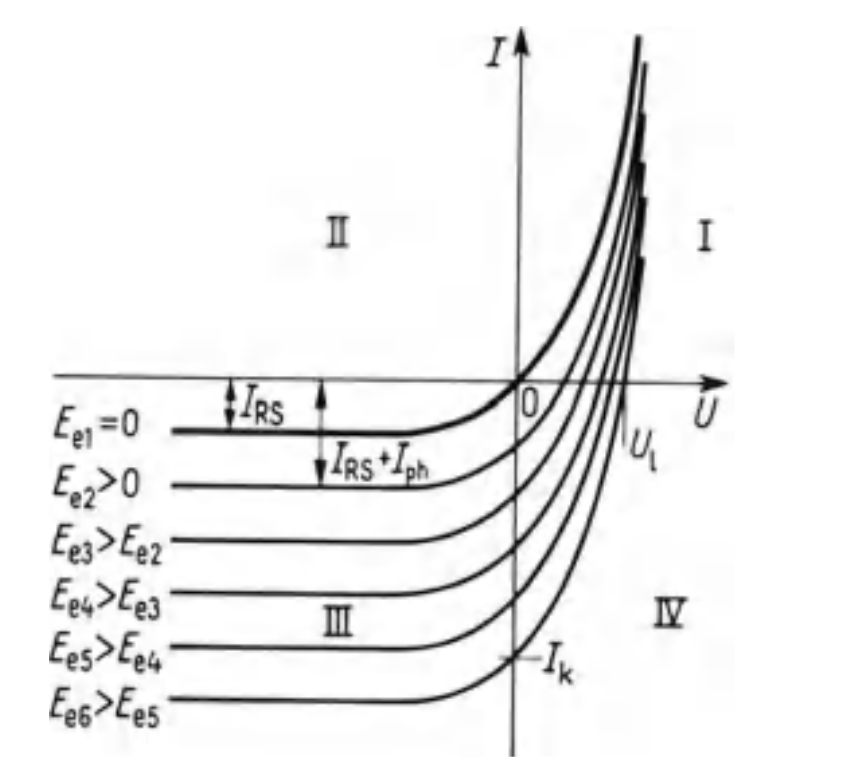
\includegraphics[width=\textwidth]{img/Photodiode-Kennline.png}
    \caption*{Kennlinienfeld $I=f(U)$ der \\Photodiode mit der Bestrah-\\lungsstärke $E_e$ als Parameter\\Kurzschlussstrom $I_k$ bei $U=0$}
    \label{fig:PhotodiodeKennline}
  \end{subfigure}
  %
  \begin{subfigure}[b]{0.6\textwidth}
    \caption{Silizium-Eindringtiefe-Licht}
    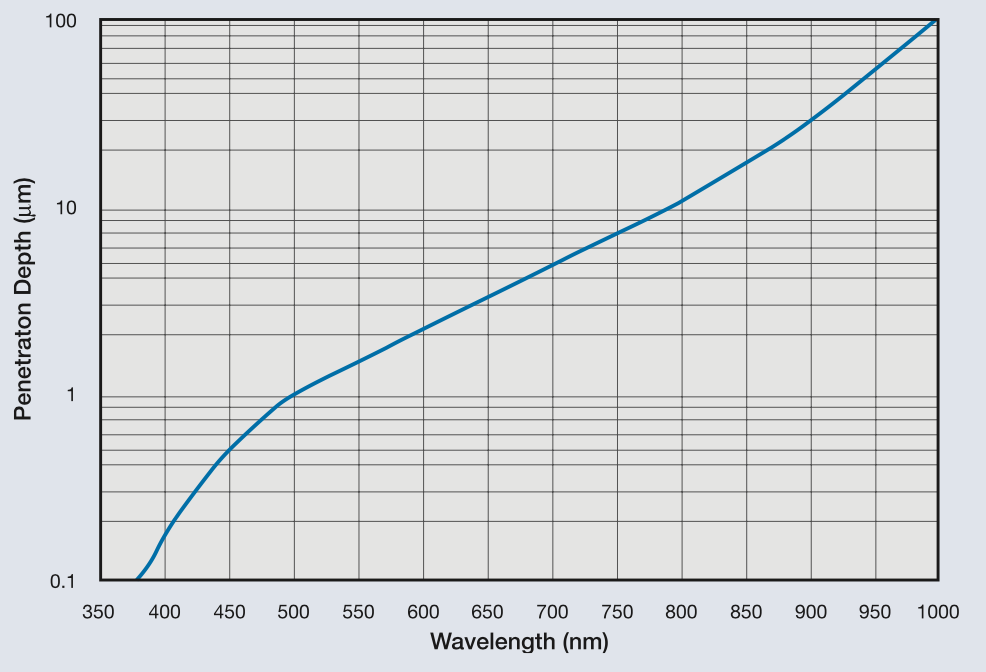
\includegraphics[width=\textwidth]{img/Silizium-Eindringtiefe-Licht.png}
    \caption*{Quelle: osioptoelectronics.com}
  \label{fig:Silizium-eindingtiefe}
  \end{subfigure}
\end{figure}







\noindent Damit Rückschlüsse über den Kurzschlussstrom $I_K$ zur Lichtintensität zulässig sind, muss also die Temperatur konstant oder zumindest bekannt sein.
Außerdem ist es wichtig, bei Tageslichtmessungen, das einfallende Licht auf eine möglichst begrenzten Wellenlängenbereich zu beschränken, da so ein möglichst akkurater Temperatur und Frequenzabhäniger kompensations faktor gewählt werden kann.
%\subsection{Analog Digital Wanlder}
\subsection{I2C}
I2C ist ein simples und effizientes Busprotokoll.
Es wurde ursprünglich von Phillips entwickelt, wird aber seit einigen Jahren von NPX weiterentwickelt.
In seiner simpelsten Form ermöglicht es einen Master mit bis zu 128 Slave-Geräten zu verbinden.
Dafür werden nur 2 Leitungen benötigt, die die SCL und SDA genannt werden. SCL ist die Taktleitung. Sie wird verwendet, um alle Datenübertragungen über den I2C-Bus zu synchronisieren. SDA ist die Datenleitung.
Außerdem müssen alle Busteilnehmer mit dem gleichen GND potential verbunden sein um Stromfluss über SDA und SCL Leitungen zu ermöglichen\footnote{www.i2c-bus.org}.


Da SCL und SDA als “open drain” betrieben werden, was bedeutet das die Busteilnehmer den Output low aber nicht high setzen können, muss ein Pull up Wiederstand zur Versorgungspannung verwendet werden.

Die Clockleitung SCL wird nur vom Bus Master gesteuert.
Die SDA Leitung wird vom Master und Slave genutzt allerdings antworten die Slaves im Normalbetrieb nur nachdem sie vom Master auf iherer Adresse eine Anfrage erhalten haben. 
Die Spezifikation des Protokolls\footnote{https://www.nxp.com/docs/en/user-guide/UM10204.pdf}  empfiehlt die SDA und SCL Leitung möglichst weit voneinander zu entfernen um so die Signalqualität zu verbessern.


